\textbf{Los Jueces y Entrenadores que tengan la misma nacionalidad pero que no se encuentren participando en
el mismo evento.}\vspace{.3cm}

\begin{center}
	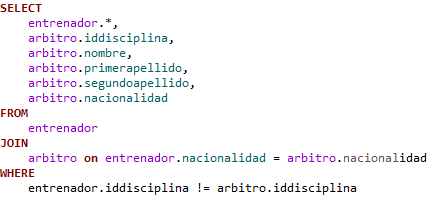
\includegraphics[width=1.05\textwidth]{resources/consulta4.png}
\end{center} 
\textbf{Explicación:} \\
Para esta consulta, seleccionamos los datos de la tabla entrenador y realizamos un join con la tabla arbitro para vincular a los entrenadores y jueces que tienen la misma nacionalidad. Luego, filtramos los resultados con la condición entrenador.iddisciplina != arbitro.iddisciplina, pues es con este dato donde se identifica si participan en el mismo evento, asegurándonos de obtener solo aquellos que, aunque compartan nacionalidad, no estén participando en el mismo evento.
 \vspace{.3cm}

\textbf{Resultado:}
\begin{center}
	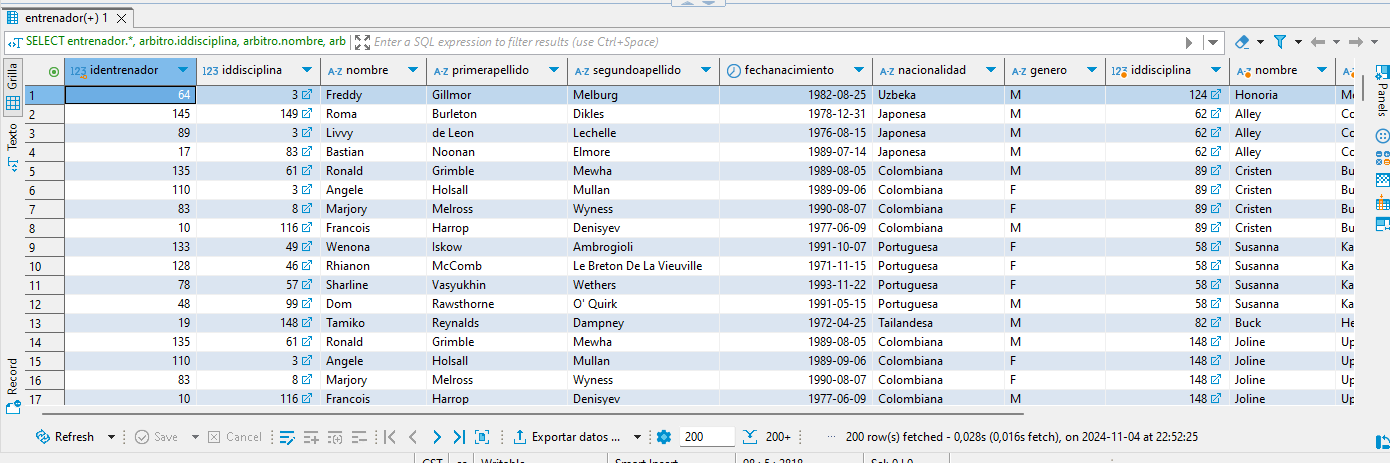
\includegraphics[width=1.05\textwidth]{resources/resultados/r4.1.png}
	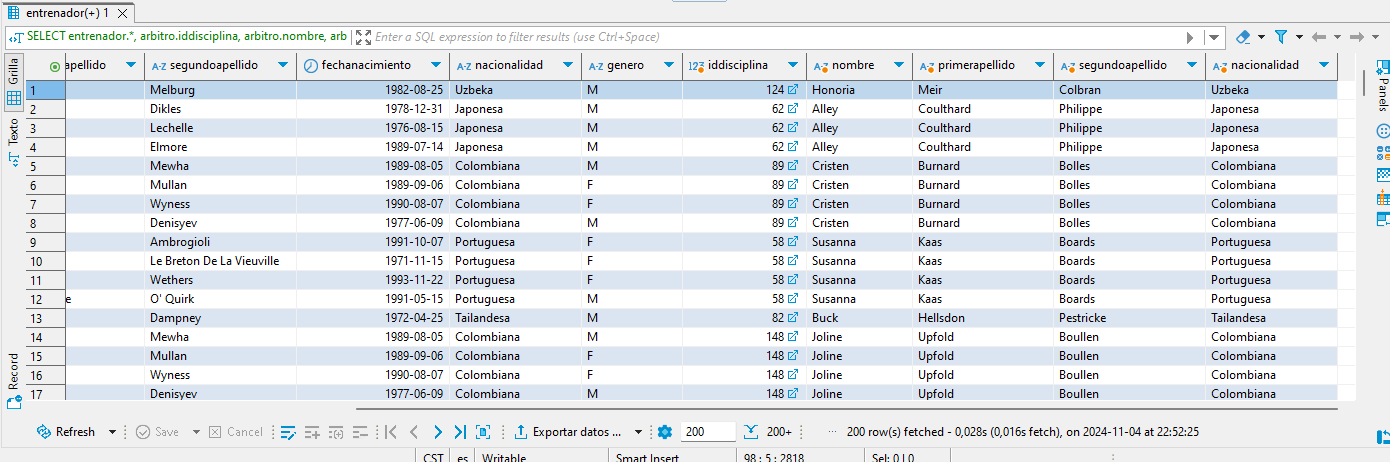
\includegraphics[width=1.05\textwidth]{resources/resultados/r4.2.png}
\end{center} 